\documentclass[11pt]{amsart}

\usepackage[letterpaper,left=125pt,right=125pt]{geometry}

% ^^^^^^^^^^^^^^^^^^^^^^^^^^^^^^^^^^^^^^^^^^^^^^^^^^^^^^^^^^^^^^^^^
\usepackage[english]{babel}
\usepackage {amsmath} 
\usepackage{amssymb}
\usepackage{amsfonts}
\usepackage{amsthm}
\usepackage{graphicx}
\usepackage[dvipsnames]{xcolor}
\usepackage{lipsum}
\usepackage[colorlinks,linkcolor=blue, citecolor=blue,urlcolor=blue]{hyperref}
\usepackage[backend=bibtex]{biblatex}
\usepackage[colorinlistoftodos]{todonotes}
\usepackage{subcaption}

\newcommand{\info}[1]{\todo[linecolor=OliveGreen,backgroundcolor=OliveGreen!25,bordercolor=OliveGreen]{#1}}
\newcommand{\unsure}[1]{\todo[linecolor=red,backgroundcolor=red!25,bordercolor=red]{#1}}
\newcommand{\change}[1]{\todo[linecolor=Plum,backgroundcolor=Plum!25,bordercolor=Plum]{#1}}

%% Environments for theorems, etc.. 
\theoremstyle{theorem} % set the style for the following theorems
\newtheorem{thm}{Theorem}[section] %\newtheorem{name}{display-text}[numbered-within]
\newtheorem{lem}[thm]{Lemma} %\newtheorem{name}[numbered-like]{display-text}
\newtheorem{cor}[thm]{Corollary}
\newtheorem{prop}[thm]{Proposition}
\newtheorem{alg}[thm]{Algorithm}
\theoremstyle{definition}       
\newtheorem{defn}[thm]{Definition}
\newtheorem{conj}[thm]{Conjecture}
\theoremstyle{example}                     
\newtheorem{prob}[thm]{Problem}
\theoremstyle{remark}                       
\newtheorem{exmp}[thm]{Example}
\newtheorem{rem}[thm]{Remark}
\newtheorem{claim}[thm]{Claim}  
\renewcommand{\theclaim}{}

\numberwithin{equation}{section}

\newcommand{\R}{\mathbb{R}}
\newcommand{\Q}{\mathbb{Q}}
\newcommand{\N}{\mathbb{N}}
\newcommand{\Z}{\mathbb{Z}}
\DeclareMathOperator{\rank}{rank}
\DeclareMathOperator{\dimension}{dim}
\DeclareMathOperator*{\supp}{supp}
\DeclareMathOperator{\spn}{span}

\newcommand\numberthis{\addtocounter{equation}{1}\tag{\theequation}}
\usepackage{mwe}

\addbibresource{wavelet.bib}

\title{Haar Wavelet and its Application in Image Compression}
\author{Jason Ngo}
\date{2019-05-03}

\begin{document}
\maketitle

\section{Introduction}
Since the start of the 20th century, we have seen rapid development in the theory and applications of wavelets. As a mathematical tool, wavelets can be used to extract information from different kinds of data such as audio signals and images. As an attempt to explore wavelets at an introductory level, this paper will examine the first wavelet developed, called the Haar Wavelet and discuss its applications in image compression.
\change{fix introduction, maybe mention where fourier series is failing and then the motivation for our wavelets.}

\info{maybe include a little bit of history of the Haar wavelet}

\begin{figure}[h]
	\centering
	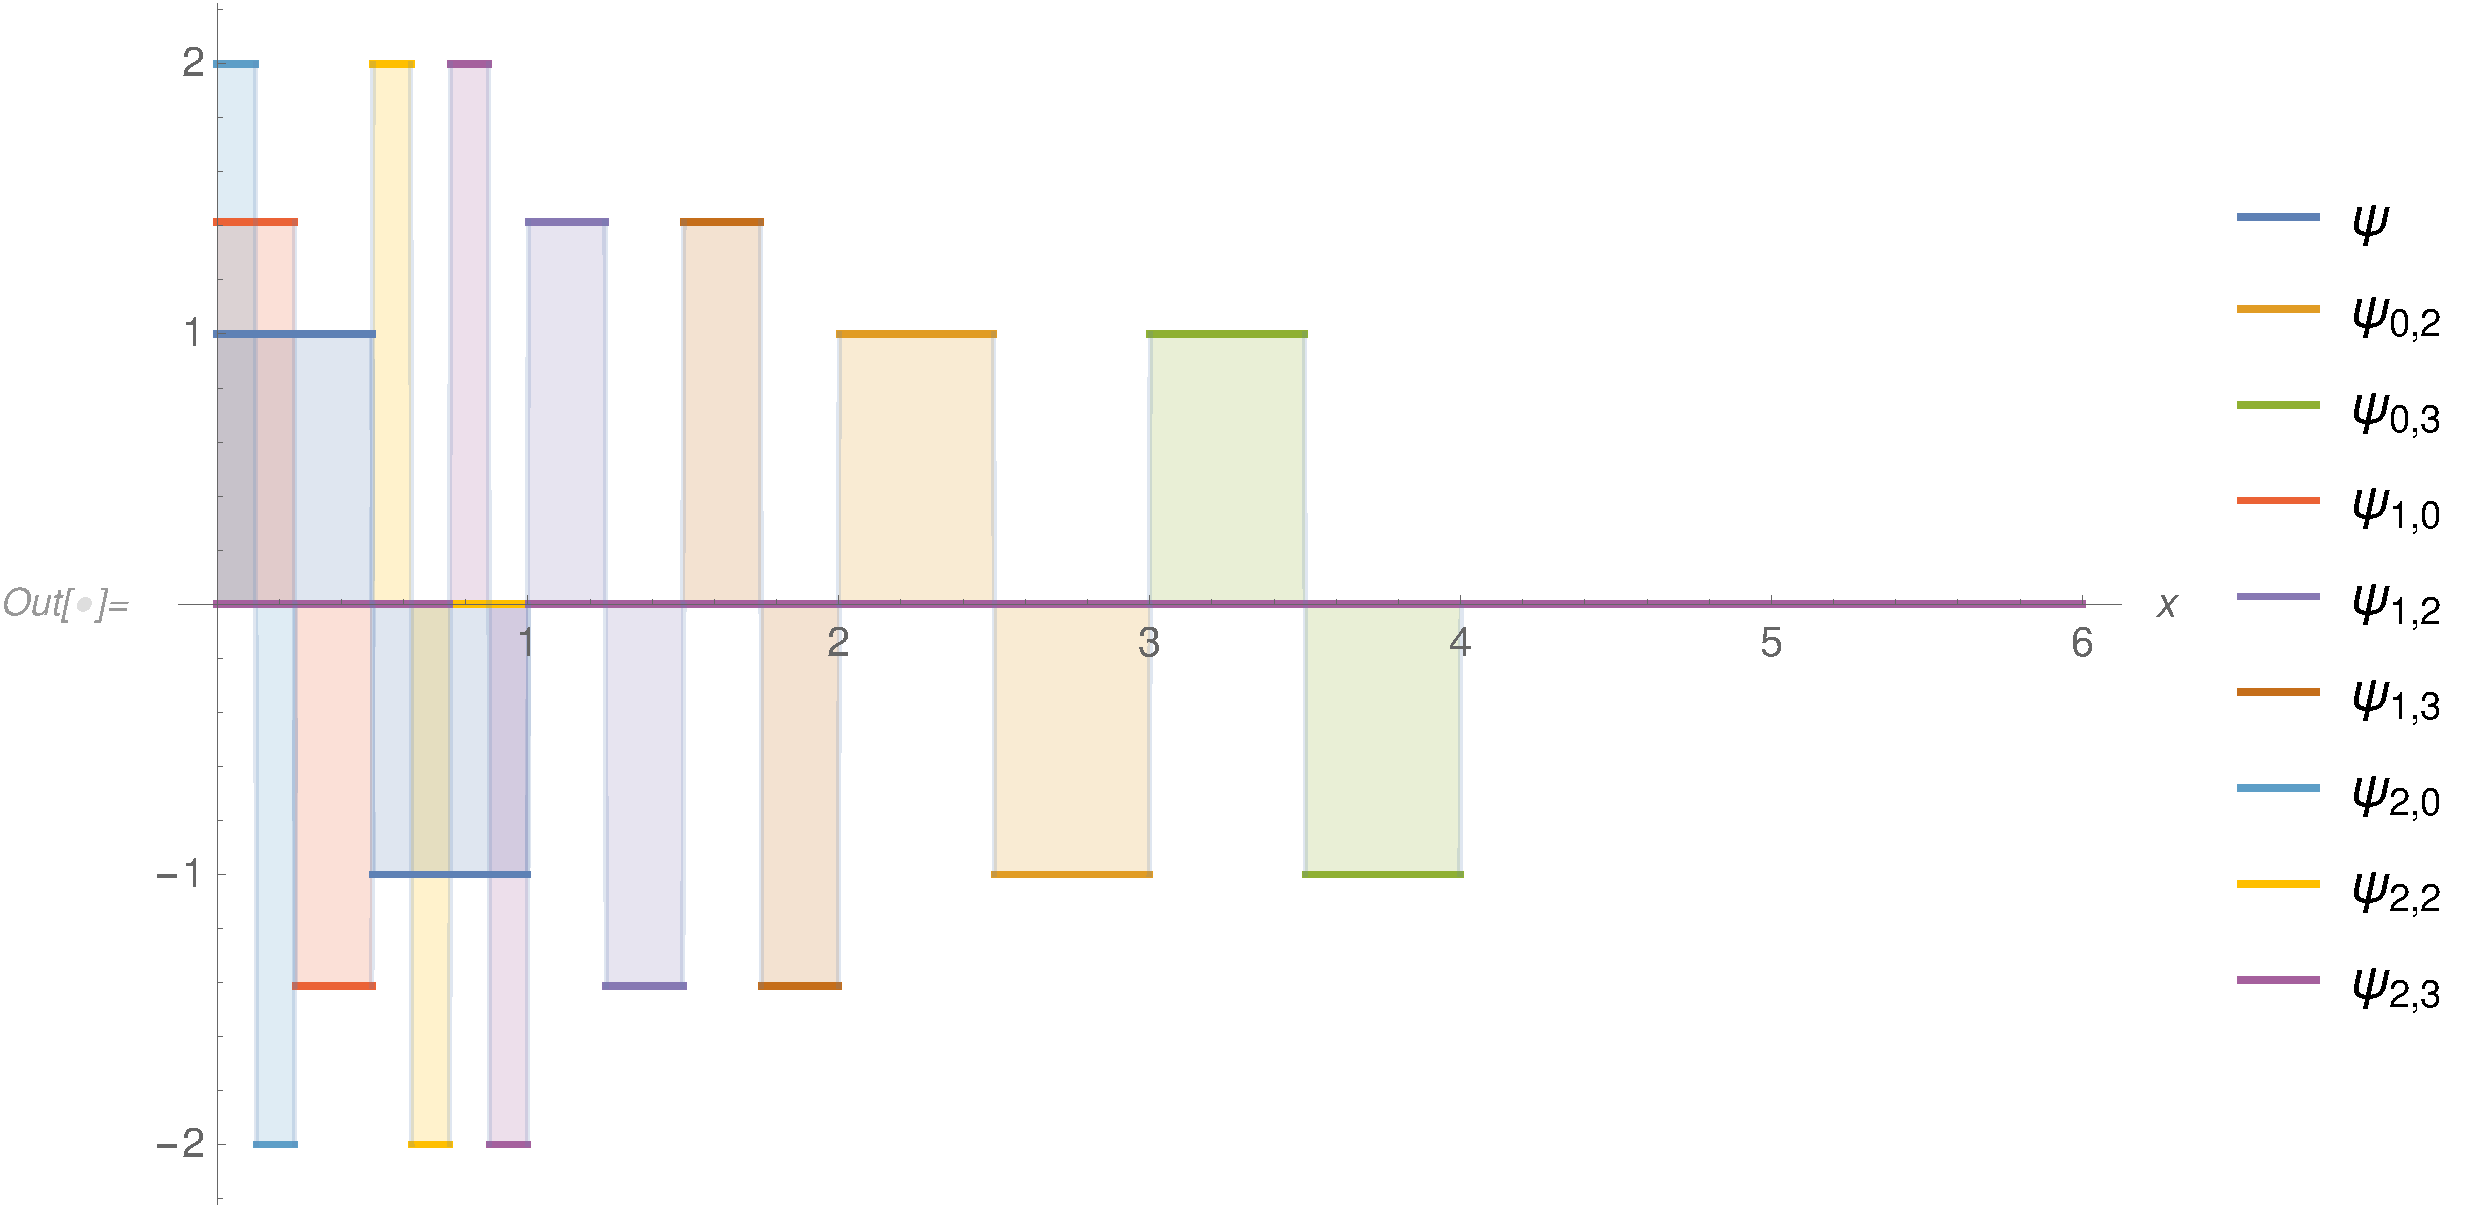
\includegraphics[width=0.7\linewidth]{img/haar_system2}
	\caption[Elements of the Haar system]{Elements of the Haar system}
	\label{fig:haarsystem}
\end{figure}


--------------

Wavelets were introduced relatively recently, in the beginning of the 1980s. 

\subsection{Motivation for Wavelets}
``Develop an important variation on Fourier series, replacing the sine and cosine functions with new families of functions, called wavelets". Want: good properties of trig functions (orthogonal basis, invariant under translation,dilation (??)).

Fourier
coefficients, and hence the Fourier series approximation, depend on all values of the
function. For example, if you change a function f a small amount on the interval
[0; 0:01], it is possible that every Fourier coefficient changes. This will then have
an effect on the partial sums $ Snf(\theta) $ for all values of $ \theta $. Although these changes
may be small, there are many subtleties in analyzing Fourier series approximations,
as we have seen.

This suggests looking for a series expansion with better local properties, meaning that coefficients reflect the local behaviour of the function and a small change
on one interval affects only a few of the series coefficients and leaves unchanged
the partial sums elsewhere in the domain. 

\section{Definition}
To get a better sense of our goals, recall that \emph{$ L^2(\R) $} is a vector space of square integrable functions, taken with the inner product
\[ \langle f,g \rangle = \int_{\R} f(x) g(x)  dx. \]

\begin{defn}[{\cite[515]{davidson}}] \label{haar}
	The \emph{Haar function} is the function $ \varPsi = \chi_{[0,0.5)} - \chi_{[0.5,1)} $. The \emph{Haar system} is the family
	\[ \{ \varPsi_{j,k}(x) = 2^{j/2} \varPsi (2^j x-k) \ | \ j,k \in \Z \}. \]
\end{defn}

	Note that each term in the Haar system is constructed by translating and/or dilating the original $ \varPsi $ (see Figure \ref{fig:haarsystem}). By this construction, since $ \int_{\R} \varPsi(x)dx = 0 $, it follows that $ \int_{\R} \varPsi_{j,k}(x)dx = 0 $ for $ j,k \in \Z $.
	Furthermore, it is important to calculate the width and height for each $ \varPsi_{j,k} $. We have $ \varPsi(2^j - k) = 1 $ when $ 0 \leq 2^j - k < \frac{1}{2} $, or equivalently, $ \frac{k}{2^j} \leq x < \frac{k+\frac{1}{2}}{2^j} $. Therefore, in this interval, $ \varPsi_{j,k} = 2^j $. Similar calculations yield:
	\begin{equation} \label{eq:height}
		\varPsi_{j,k} = 
		\begin{cases}
		2^{j/2} &\text{if}\ \frac{k}{2^j} \leq x < \frac{k+\frac{1}{2}}{2^j}, \\
		-2^{j/2} &\text{if}\ \frac{k+\frac{1}{2}}{2^j} \leq x < \frac{k+1}{2^j}, \\
		0 &\text{otherwise}.
		\end{cases}
	\end{equation}
	
Now, we will prove that the Haar function $ \varPsi $ satisfies Definition \ref{def:wavelet} of an \emph{orthonormal wavelet}.

\begin{defn}[Orthonormal Wavelet, {\cite[303]{pinsky}}] \label{def:wavelet}
	If $ \varPsi \in L^2(\R) $, $ \varPsi_{j,k}(x) = 2^{j/2} \varPsi (2^j x-k) $, and the set $ \{ \varPsi_{j,k}: j,k \in \Z \} $ is an orthonormal basis for $ L^2(\R) $, then $ \varPsi $ is called an \emph{orthonormal wavelet}.
\end{defn}

To prove the Haar system is an \textit{orthonormal basis}, we have to show:
	\begin{enumerate}
		\item The Haar system $ \{ \varPsi_{j,k} \} $ is an orthonormal set, i.e. $ \| \varPsi_{j,k} \| = 1 $ for all $ j,k \in \Z $ and $ \langle \varPsi_{j,k}, \varPsi_{j',k'} \rangle = 0 $ for all $ (j,k) \neq (j',k') $.
		
		\item The span of Haar system, denoted $ \spn\{\varPsi_{j,k}\} $, is dense in $ L^2(\R) $.
	\end{enumerate}

In Section \ref{section:orthonormality}, we will first prove that the Haar system is orthonormal. Section \ref{section:span} will show that it spans a dense subspace of  $ L^2(\R) $. Finally, in Section \ref{section:application}, we will discuss the Haar wavelet's local property and its application in image compression.

\section{Orthonormality} \label{section:orthonormality}
To get started, building upon the terse proof in  \cite{davidson}, this section proves that the Haar system is orthonormal, followed by a short discussion of the normalization factor.

\begin{lem}[{\cite[409]{davidson}}] \label{lem:orthonormal}
	The Haar system is an orthonormal set in $ L^2(\R) $.
	
	\begin{proof}
		First, it is easy to see that $ \| \varPsi \| = 1 $. Let us compute:
		\begin{align*}
		\| \varPsi_{j,k} \|^2 = \int_{\R} \left| 2^{j/2} \varPsi(2^{j} x - k) \right|^2 dx 
		&=   \int_{\R} 2^j \left| \varPsi(2^{j} x - k) \right|^2 dx \\
		&= \int_{\R} \left| \varPsi(y) \right|^2 dy
		= \| \varPsi \|^2,
		\end{align*}
		by change of variable $ y = 2^{j}x-k $ in the integral. Therefore, all the elements in the Haar system has norm 1.
		
		Now, we want to show the orthogonality. Consider $ \varPsi_{j,k} $ and $ \varPsi_{j,k'} $, for $ k \neq k' $. Since these two elements have disjoint support\footnote{The \emph{support} of a function, denoted $ \supp $, is the subset of the domain containing those elements which are not mapped to zero.}, their inner product is 0. If $ j < j' $, then either $ \varPsi_{j,k} $ and $ \varPsi_{j',k'} $ have disjoint supports (when $ k \neq k' $), or supp $ \varPsi_{j',k'} $ is contained in an interval on which $ \varPsi_{j,k} $ is constant to $ 2^{j/2} $ (when $ k = k' $). For the former case, their inner product is obviously 0; for the latter case, we have:
		\[ \langle \varPsi_{j,k}, \varPsi_{j',k'} \rangle =  \int_{\R} 2^{j/2} \cdot \varPsi_{j',k'} dx = 2^{j/2} \int_{\R} \varPsi_{j',k'} dx = 0. \]
	
		Hence, the set is orthonormal.
	\end{proof}
\end{lem}

\begin{rem}
	The Haar function is a dyadic function, meaning that the dilations are taken to be powers of 2. Here, the factor $ 2^{j/2} $ is called the normalization factor, which is there so that the dilated and translated Haar function has norm 1. Although powers of 2 are a common choice, they are certainly not the most general one\footnote{See examples of non-dyadic wavelets and a discussion why they are more appropriate for statistical data analysis in \cite{pollock}.}.
\end{rem}

%Now that we have proved the Haar system is orthonormal, Section \ref{section:span} will finish proving the Haar function satisfies Definition \ref{def:wavelet}.

\section{Haar Wavelet Basis for $ L^2(\R) $} \label{section:span}
Now that we have shown the Haar system is orthonormal, this section will finish showing $ \varPsi $ satisfies Definition \ref{def:wavelet} by proving the following theorem:

\begin{thm}[{\cite[411]{davidson}}] \label{thm:span}
	The Haar system $ \{ \varPsi_{j,k} \} $ spans all of $ L^2(\R) $.
\end{thm}

To prove this theorem, we will start out with $ C_c(\R) $, the set of continuous functions with compact support. Since $ C_c(\R) $ is dense in $ L^2(\R) $\footnote{The proof that $ C_c(\R) $ is dense in $ L^2(\R) $ can be found in \cite[326]{farrell}.}, if we can show that any function $ f \in C_c(\R) $ is in the closure of the span of $ \{\varPsi_{j,k}\} $, then it follows that $ \{ \varPsi_{j,k} \} $ spans $ L^2(\R) $.

Motivated by \cite[3]{bell} and \cite[516]{davidson}, we will set up the integral transform $ P_nf $ in Section \ref{subsec:integral transform}, and then proceed to define the Haar inner product expansion in Section \ref{subsec:two-sided}, which indeed can approximate any function in $ C_c(\R) $.
%If we can show that this expansion of the Haar system covers $ C_c(\R) $, then we have successfully proved Theorem \ref{thm:span}.

\subsection{Integral Transform} \label{subsec:integral transform}

\vspace{8pt}
Set $ \phi(x) = \chi_{[0,1)}$. For $ n \in \Z $, we define the integral kernel
\[ K_n (x,y) = 2^n \sum_{k \in \Z} \phi(2^n x - k) \phi(2^n y - k). \]

Note that $ K_n $ is either equal to $ 2^n $ (when there is some $ k \in \Z $ s.t. $ 2^n x-k $ and $ 2^ny - k $ lie in $ [0,1) $) or equal to 0 (otherwise). In other words, if $ K_n = 2^n $, then there is some $ k $ s.t.
\begin{equation} \label{eq:K}
	x,y \in \left[ \frac{k}{2^n}, \frac{k+1}{2^n} \right) = I_{n,k}.
\end{equation}

Here, note that each $ I_{n,k} $ has length $ 2^{-n} $ and that
%$ K_n(x,y) $ is constant (equal to $ 2^n $) on each dyadic interval of length $ 2^{-n} $. Furthermore, for any given $ n \in \Z $, 
the sets $ \{ I_{n,k} \} $ are disjoint.

We define the integral transform
\[ P_n f(x) = \int_{\R} K_n(x,y) f(y) dy. \]
If $ x \in \R $ then there is a unique $ k_x \in \Z $ with $ x \in I_{n, k_x} $ and
\begin{equation} \label{eq:pnf}
	P_n f(x) = 2^n \int_{I_{n,k_x}} f(y) dy.
\end{equation}
Since $ I_{n,k_x} $ has length $ 2^{-n} $, we can say that $ P_nf $ is the average value of a function $ f $ on the dyadic interval containing $ x $.

\vspace{8pt}
Notice that the integral kernel $ K_n $ is dependent on $ \phi $. In order to write any function in terms of the Haar system $ \{ \varPsi_{j,k} \} $, we must eliminate $ \phi $ somehow from our calculations. The following Lemma \ref{lem:expansion} will write the integral kernels in terms of $ \{ \varPsi_{j,k} \} $.

\begin{lem}[{\cite[293]{pinsky}}] \label{lem:expansion}
	If $ n \in \Z $, then
	\[ K_{n+1} - K_n = \sum_{k \in \Z} \varPsi_{n,k}(x) \varPsi_{n,k}(y),\qquad x,y \in \R. \]
	
	\begin{proof}
		First, let us calculate the right-hand side.
		By Equation (\ref{eq:height}), $ \varPsi_{n,k}(x) = 2^{n/2} $ when $ x \in I_{n+1,2k} = \left[\frac{2k}{2^{n+1}}, \frac{2k+1}{2^{n+1}}\right) $, and similarly, $\varPsi_{n,k}(x)= -2^{n/2} $ when $ x \in I_{n+1,2k+1}$. Therefore, it follows that:
		\[
		\varPsi_{n,k}(x) \varPsi_{n,k} (y) =
		\begin{cases}
		2^n &\text{if}\ x,y \in I_{n+1,2k}\ \text{or}\ x,y \in I_{n+1,2k+1}, \\
		-2^n &\text{if one is in }\ I_{n+1,2k}\ \text{and the other is in}\ I_{n+1,2k+1}, \\
		0 &\text{otherwise}.
		\end{cases}
		\]
		
		Now, before calculating the left-hand side $ K_{n+1} - K_n $, note that:
		\[
		I_{n+1,2k} \cup I_{n+1,2k+1} = \left[ \frac{2k}{2^{n+1}}, \frac{2k+2}{2^{n+1}} \right) = I_{n,k}. 
		\]
		
		Therefore, if both $ x,y $ are in $ I_{n+1,2k} $ or $ I_{n+1,2k+1} $, then we have (1) $ K_{n+1} = 2^{n+1} $ (by Equation (\ref{eq:K})) and (2) $ K_n = 2^n $ (because $ x,y \in I_{n,k} $), Hence,
		\[ K_{n+1}(x,y) - K_n(x,y) = 2^{n+1} - 2^n = 2^n. \]

		By similar argument, if either $ x $ or $ y $ is in $  I_{n+1,2k} $ and the other is in $ I_{n+1,2k+1} $, then
		$ K_{n+1}(x,y) - K_n(x,y) = 0 - 2^n = -2^n. $ Otherwise, both $ K_{n+1} $ and $ K_n $ are 0.
		
		Thus, we conclude $ K_{n+1}(x,y) - K_n(x,y) = \sum_{k \in \Z} \varPsi_{n,k}(x) \varPsi_{n,k}(y) $.
	\end{proof}
\end{lem}

\vspace{8pt}
\begin{rem}
	From this Lemma, the difference between two integral transforms can be written as the \textit{inner product expansion} of the function $ f $:
	\begin{align*}
	(P_{n+1} - P_n) f(x) &= \int_{\R} K_{n+1}(x,y)f(y)dy - \int_{\R} K_{n}(x,y)f(y)dy \\
	&= \int_{\R} \sum_{k \in \Z} \varPsi_{n,k}(x) \varPsi_{n,k}(y) f(y) dy \\
	&= \sum_{k \in \Z} \varPsi_{n,k}(x) \int_{\R} \varPsi_{n,k}(y) f(y) dy \\
	&= \sum_{k \in \Z} \langle f, \varPsi_{n,k} \rangle \varPsi_{n,k}(x).  \numberthis \label{eq:expansion}
	\end{align*}
	
	The terms $ \langle f, \varPsi_{j,k} \rangle $ are called the the Haar coefficients.
	One can easily notice that this inner product expansion is only one-sided, meaning we keep the dilation factor $ j = n $ fixed and vary the translation factor $ k $. In the next section, we will abstract this expansion to a more general setting, varying both the translation and dilation factors.
\end{rem}


\subsection{Two-sided Haar Representation} \label{subsec:two-sided}
From Equation \ref{eq:expansion}, we can write
\begin{equation} \label{eq:twosided}
	P_{n+1}f(x) - P_{-m}f(x) = \sum_{j=-m}^{n} \sum_{k \in \Z} \langle f, \varPsi_{j,k} \rangle \varPsi_{j,k}(x).
\end{equation}

To prove that any function $ f \in C_c(\R) $ is in the closure of the span of $ \{ \varPsi_{j,k} \} $, we want to show that the Haar inner product expansion on the right-hand side converges to $ f $. Fortunately, we can do so by showing that $ P_{-m}f \to 0 $ and $ P_{n+1}f \to f $ with respect to the $ L^2 $ norm as $ m, n \to \infty $. The two claims are presented as Lemmas below.

\vspace{8pt}
First, Lemma \ref{lem:average} tells us that the larger the intervals on which we average a continuous function, the smaller the supremum of the averaged function.

\begin{lem}[Average Function over Dyadic Intervals, {\cite[295]{pinsky}}] \label{lem:average}
	If $ f \in C_c(\R) $, then $ \|P_{-m}f\|_2 \to 0 $ when $ m \to \infty $.
	
	\begin{proof}
		Suppose $ f \in C_c(R) $ and $ \supp(f) \subseteq [-K,K] $. There eixsts $ M > 0 $ s.t. $ \supp(f) \subset [-2^M, 2^M] $. Now, if $ m > M $, then $ \supp(f) \subseteq I_{-m,-1} \cup I_{-m,0} $; Equation (\ref{eq:pnf}) therefore holds.
		We compute:
		\begin{align*}
			\| P_{-m}f \|_2^2 &= \int_{\R} \left| P_{-m}f(x) \right|^2 dx 
			= \sum_{k \in \Z} \int_{I_{-m,k}} |P_{-m}f(x)|^2 dx \\
			&= \sum_{k \in \Z} \int_{I_{-m,k}} \left|2^{-m} \int_{I_{-m,k}} f(y) dy \right|^2 dx
%			 \qquad \text{(by (\ref{eq:pnf}))} \\
%			&
			= 2^{m}  2^{-2m} \sum_{k \in \Z} \left|\int_{I_{-m,k}} f(y) dy \right|^2 dx.
		\end{align*}
		Since $ f $ is only supported on a subset of $ I_{-m,-1} $ and $ I_{-m,0} $, we have:
		\begin{align*}
		\| P_{-m}f \|_2^2	&= 2^{-m} \left( \left|\int_{I_{-m,-1}} f(y) dy \right|^2 dx + \left| \int_{I_{-m,-1}} f(y) dy \right|^2 dx \right) \\
			&=  2^{-m} \left( \left|\int_{-K}^0 g(y) dy \right|^2 dx + \left| \int_{0}^K f(y) dy \right|^2 dx \right).
		\end{align*}
		Note that $ \int_{-K}^0 f(y) dy = \langle f(y),\chi_{[-K,0)}  \rangle $; by Cauchy-Schwarz inequality,
		\begin{align*}
		\| P_{-m}f \|_2^2	&\leq  2^{-m} \left( K \|f\|_2^2 + K \|f\|_2^2 \right) = 2^{-m} \cdot 2K \|f\|_2^2.
		\end{align*}
		As $ m \to \infty $, the right-hand side converges to 0. Therefore, by Squeeze Theorem, it follows that $ \|P_{-m}f\|_2 \to 0 $.
	\end{proof}
\end{lem}

Now, before proving our next Lemma, recall that $ P_nf(x) $ is equal to the average value of a function $ f $ on a small dyadic interval of length $ 2^{-n} $. Therefore, if we increase $ n $, then the intervals will get smaller, and the average value $ P_nf $ will get closer to $ f $ (see Figure \ref{fig:converge} for the sequence $ \{P_nf\} $ approaching $ f(x) = e^{-x} \sin{2\pi x} $ on the unit interval). 
\info{This Lemma is particularly useful in signal denoising: given a time series, we} 

\begin{figure}[h]
	\centering
	\begin{subfigure}[b]{0.475\textwidth}
		\centering
		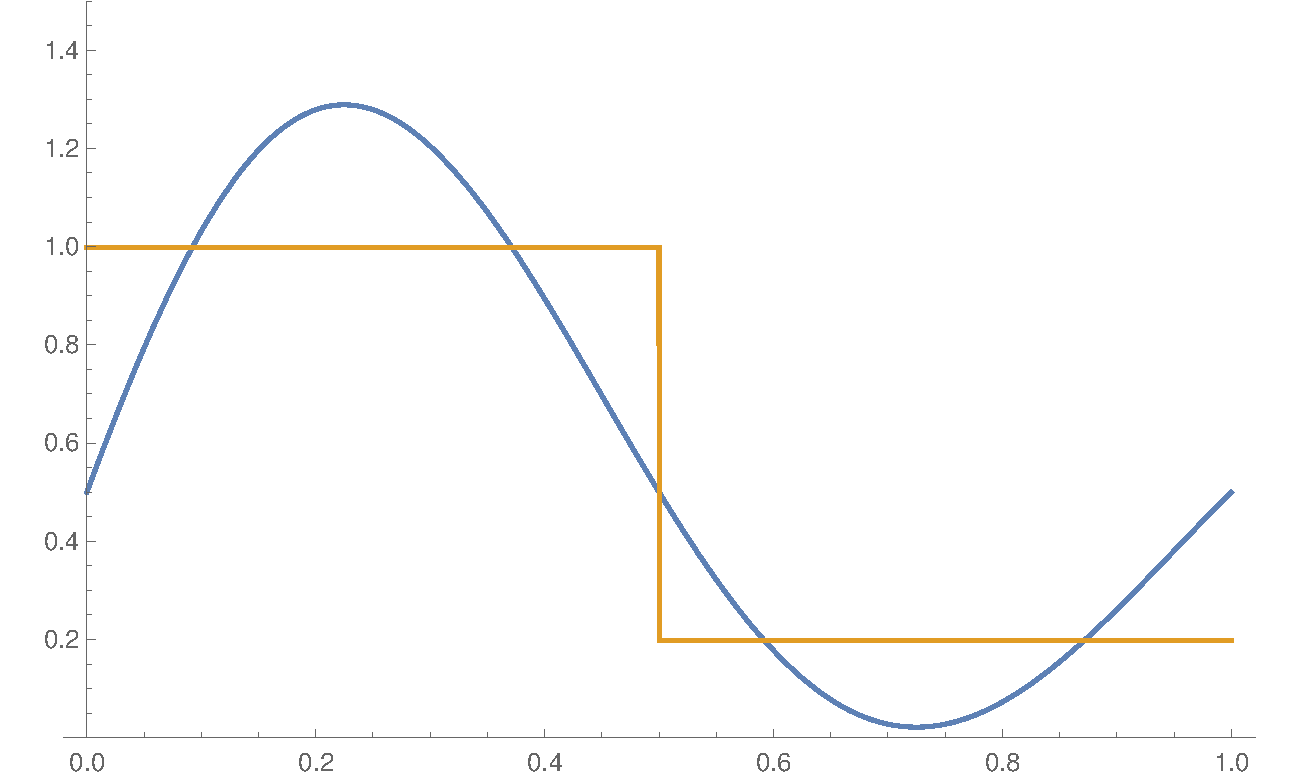
\includegraphics[width=\textwidth,height=0.4\linewidth]{img/e1}
		\caption[Network2]%
		{{\small $ n = 1 $}}    
	\end{subfigure}
	\hfill
	\begin{subfigure}[b]{0.475\textwidth}  
		\centering 
		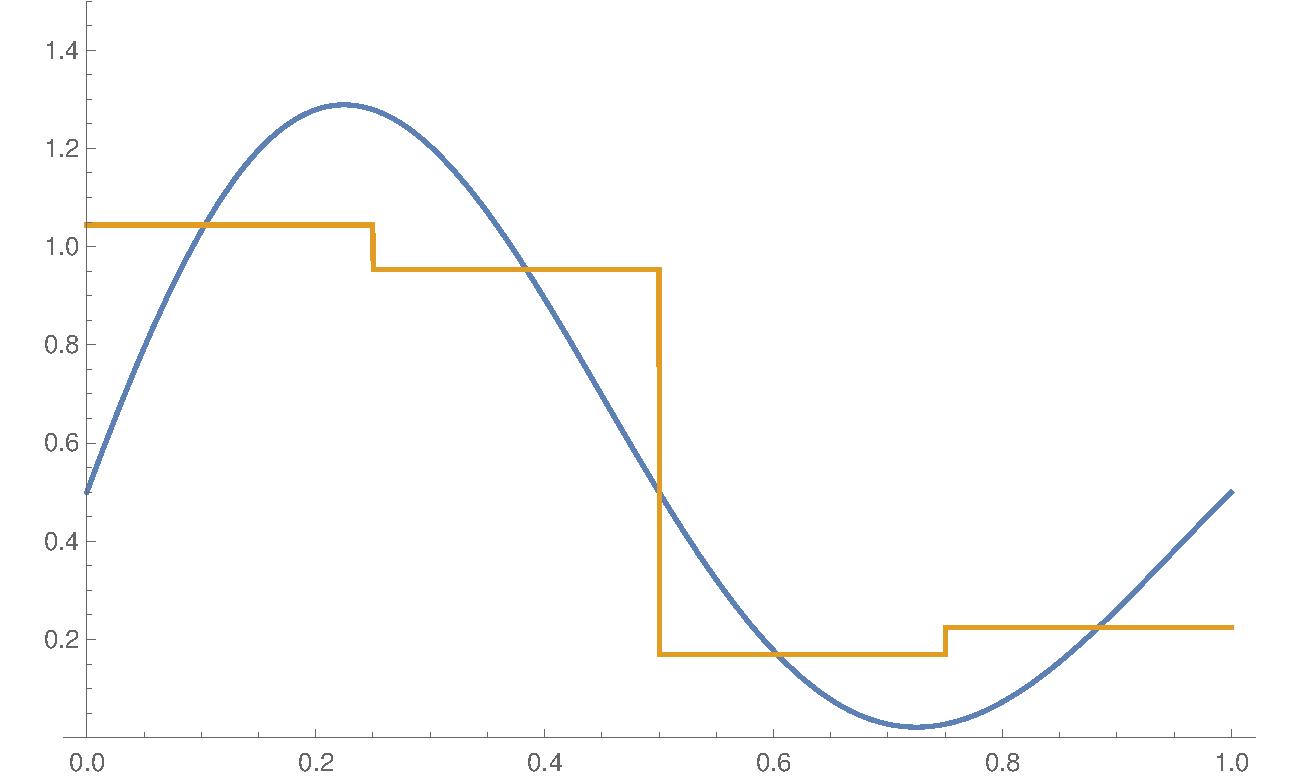
\includegraphics[width=\textwidth,,height=0.4\linewidth]{img/e2}
		\caption[]%
		{{\small $ n = 2 $}}
	\end{subfigure}
	\vskip\baselineskip
	\begin{subfigure}[b]{0.475\textwidth}   
		\centering 
		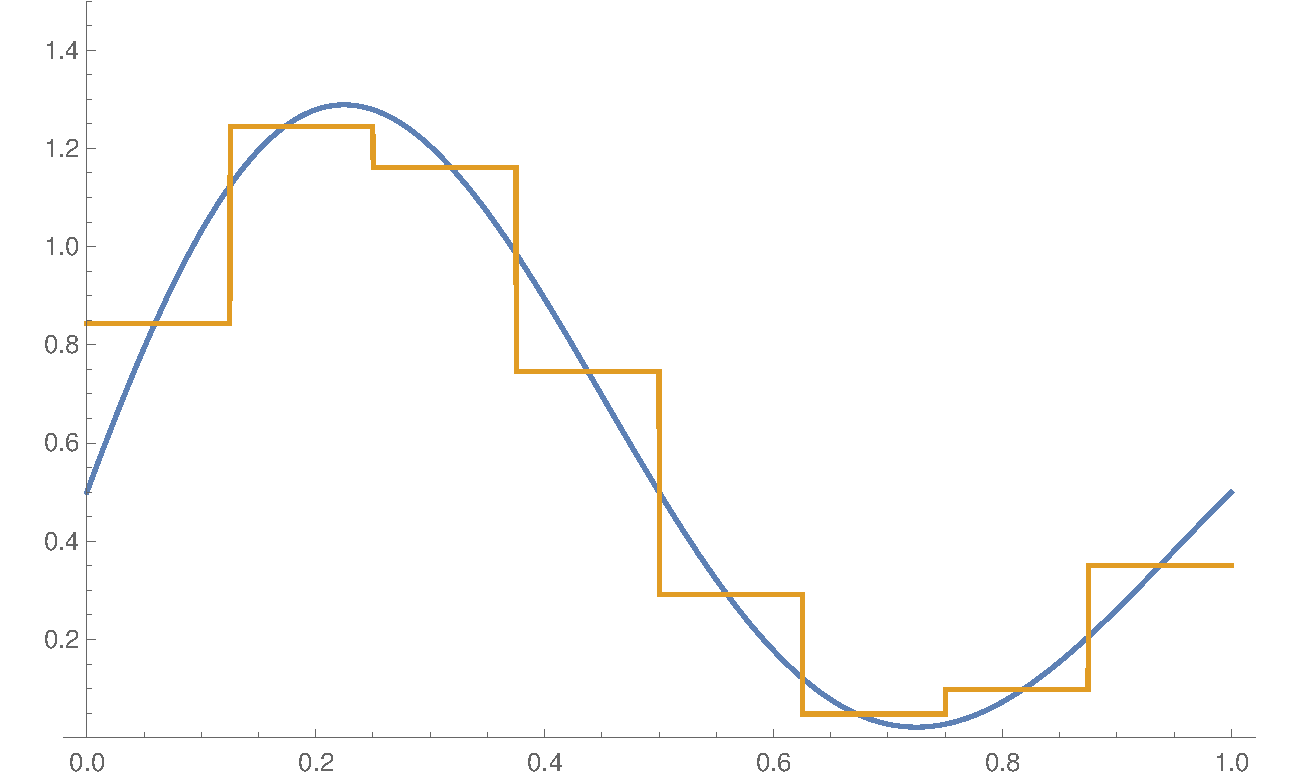
\includegraphics[width=\textwidth,,height=0.4\linewidth]{img/e3}
		\caption[]%
		{{\small $ n = 3 $}}    
	\end{subfigure}
	\quad
	\begin{subfigure}[b]{0.475\textwidth}   
		\centering 
		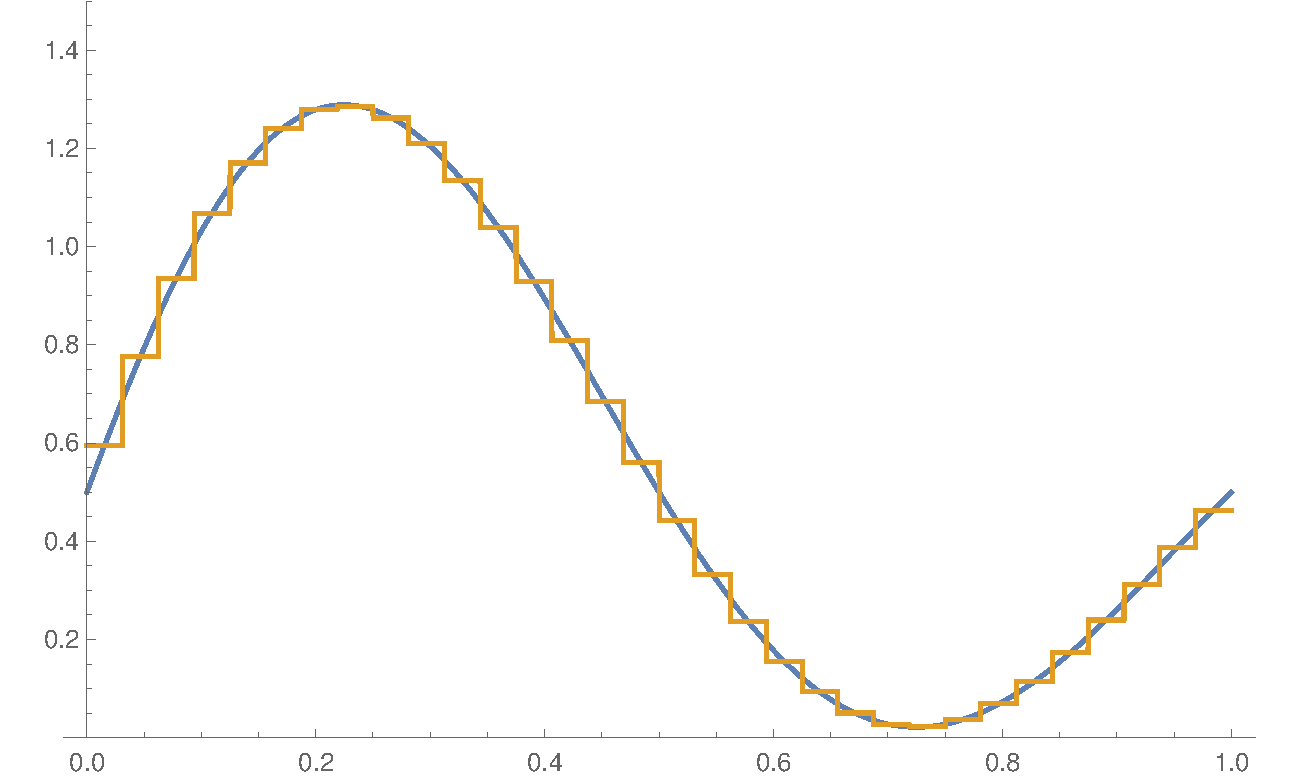
\includegraphics[width=\textwidth,height=0.4\linewidth]{img/e5}
		\caption[]%
		{{\small $ n = 5 $}}    
	\end{subfigure}
	\caption[]
	{Approximation of $ f(x) = e^{-x} \sin{2\pi x} $ by $ P_nf(x) $}
	\label{fig:converge}
\end{figure}

\begin{lem}[Convergence of Integral Transform, {\cite[517]{davidson}}] \label{lem:convergence}
	If $ f \in C_c(\R) $, then $ P_nf \to f $ in the uniform norm as well as in the $ L^2 $ norm.
	
	\begin{proof}
		Suppose $ f \in C_c(\R) $ and $ \supp(f) \subset [-2^M, 2^M] $ for $ M \geq 0 $. Since $ f $ is continuous on a compact set, it is uniformly continuous.
		
		Given $ \epsilon > 0 $. By uniform continuity, there exists $ \delta > 0 $ such that if $ |x-y| < \delta $, then $ |f(x) - f(y)| < \epsilon $.
		
		Now, choose $ N $ such that $ 2^{-N} < \delta $; if $ n > N $, then we have:
		\begin{align*}
		|P_nf(x) - f(x)| &= \left| 2^n \int_{I_{n,k_x}} f(y)dy - f(x) \right| \\
		&=  \left| 2^n \int_{I_{n,k_x}} f(y)dy - 2^n \int_{I_{n,k_x}} f(x) dy \right| \\
		&\leq 2^n \int_{I_{n,k_x}} |f(y) - f(x)| dy 
		< 2^n \int_{I_{n,k_x}} \epsilon dy = \epsilon.
		\end{align*}
		Therefore, $ P_nf $ converges to $ f $ uniformly. Since uniform convergence implies $ L^2 $ convergence, it follows that $ P_nf \to f $ with respect to the $ L^2 $ norm.
	\end{proof}
\end{lem}

\vspace{8pt}
Now, by Lemma \ref{lem:average} and Lemma \ref{lem:convergence}, it follows that for any $ f \in C_c(\R) $, 
	\[
	f = \sum_{j \in \Z} \sum_{k \in \Z} \langle f, \varPsi_{j,k} \rangle \varPsi_{j,k}.
	\]
Since $ C_c(\R) $ is a dense subspace of $ L^2(\R) $, we conclude that the Haar system spans $ L^2(\R) $. The Haar function $ \varPsi $ is therefore an orthonormal wavelet.\qed

\info{maybe i can compare and contrast haar wavelet basis versus fourier series. draw some more graphs and that's it. to see how much more useful haar wavelet basis is.}


\section{title}
\change{pls fix}
GRAPH THE COEFFICIENTS
A good feature of the Haar wavelets can be noticed. By increasing the wavelet number, the wavelet coefficients rapidly decrease and higher coefficients are practically zero. --> can confine to a small number of terms in the wavelet series.

Tie back to the motivation at the beginning of the paper

%; we will now refer to it as the \emph{Haar wavelet}.
%\change{if i decide to add application, then delete this, if not then keep it}

%\section{Application to Image Compression} \label{section:application}
%\change{this section is a mess}
%In this section, we discuss image compression as an application of the Haar wavelet basis. First, we define what we mean by compression. When compressing images, we want to discard the least significant details, keeping the original picture largely intact. Since an image is two-dimensional, it is helpful to think of image compression as discarding least significant details from the sets of row pixels and column pixels. 
%
%For instance, suppose we are given a function $ f(x) $ expressed in terms of span of basis functions $ \{ u_i \} $:
%	\[ f(x) = \sum_{i=0}^{M-1} c_i u_i(x). \]
%The data set in this case consists of the coefficients $ c_i $. We would like to find a function approximating $ f(x) $ but requiring fewer coefficients, perhaps by using a different basis.
%
%Because Haar wavelet basis is orthonormal, we can easily calculate the coefficients and sort them in decreasing magnitude. Furthermore, due to its highly localization (the support for each function is located in a narrow dyadic interval), small coefficients can be discarded without losing much data.
%
%\begin{figure}[h]
%	\centering
%	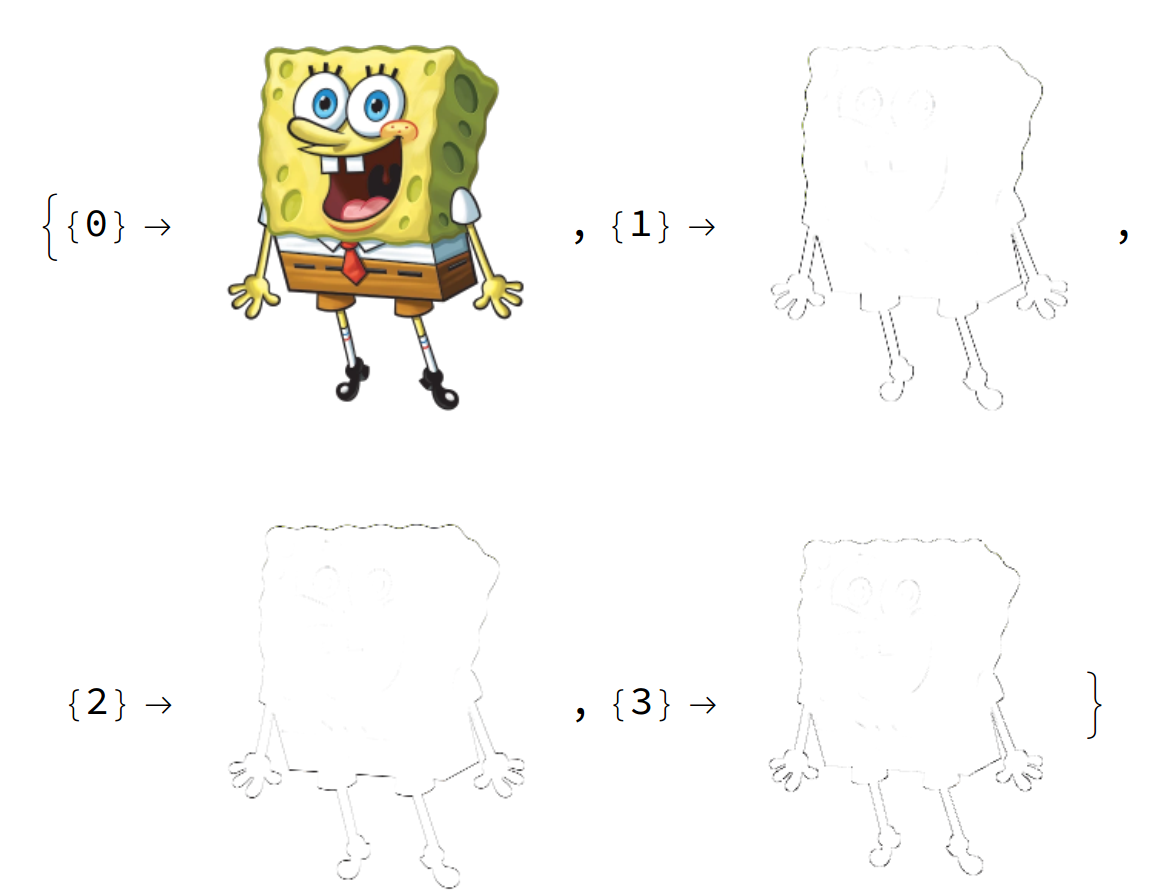
\includegraphics[width=0.7\linewidth]{img/s.png}
%	\caption{Compression with Haar Wavelet Basis}
%	\label{fig:s2}
%\end{figure}
%
%Figure \ref{fig:s2} shows the four most significant coefficients when we apply image compression using Haar Wavelet Basis. The implementation of this compression algorithm can be found in \cite{stollnitz}.

\printbibliography

\end{document}

